% Chapter Template

\chapter{Understanding Human Motion} % Main chapter title

\label{Chapter3} % Change X to a consecutive number; for referencing this chapter elsewhere, use \ref{ChapterX}

\lhead{Chapter 3. \emph{Understanding Human Motions}} % Change X to a consecutive number; this is for the header on each page - perhaps a shortened title

 Human motions are rich in information. It conveys to the receiver the emotion, the attitude, the deeds and even the health of the human. Without understanding completely the human motion, it is not possible to achieve a very good interaction system.  Vision based motion capture and analysis has been studied widely and for instance a condensed summary of all the approaches developed during the past two decades until 2000 have been presented by Moeslund et al. in \cite{Moeslund2001231} followed by the study of advancements during the years 2000-2006 in the survey \cite{Moeslund200690}. In the former the authors reviewed more than 130 publications while in the latter a review of over 300 publications was presented. This shows the rapid advancements in the study of the human motion in the recent times. Another work by Ronald Poppe\cite{Poppe20074} on the overview of vision based human motion analysis approached the problem into two discrete problems of modeling and estimation while also discussing the model free approaches to motion analysis. In this chapter an overview of the various approaches for pose estimation from RGB-D data and the gesture recognition are covered.
%----------------------------------------------------------------------------------------
%	SECTION 1
%----------------------------------------------------------------------------------------
%\section{Human Body models}
%\label{sec:humanmodel}
%	The human motion understanding is incomplete without understanding the kinematic model of the human body. Human body is by far the most complex system in terms of its composition. Human body models describe both the kinematic properties of the body (the skeleton), as the shape and appearance(the flesh and skin). Most of the models describe the human body as a kinematic tree, consisting of segments that are linked by joints. Every joint contains a number of degrees of freedom (DOF), indicating in how many directions the joint can move. All DOF in the body model together form the pose representation. These models can be described in either 2D or 3D. 2D models are suitable for motion parallel to the image plane and are sometimes used for gait analysis but are not sufficient for analysis of more complex motions. 3D models most often model segments as rigid, and allow a maximum of three (orthogonal) rotations per joint and for each of the rotations individually, kinematic constraints can be imposed. The number of DOF considered in the literature varies from 10 DOF to as much as 50 DOF. However we would see in the section~\ref{sec:humanpose} that the pose estimation approaches identifies between 16$\sim$25 joints. Some of the most commonly used human kinematic models for motion analysis are shown in Figure~\ref{fig:humkinmodel}. 
%
%\begin{figure}[H]
%\centering
%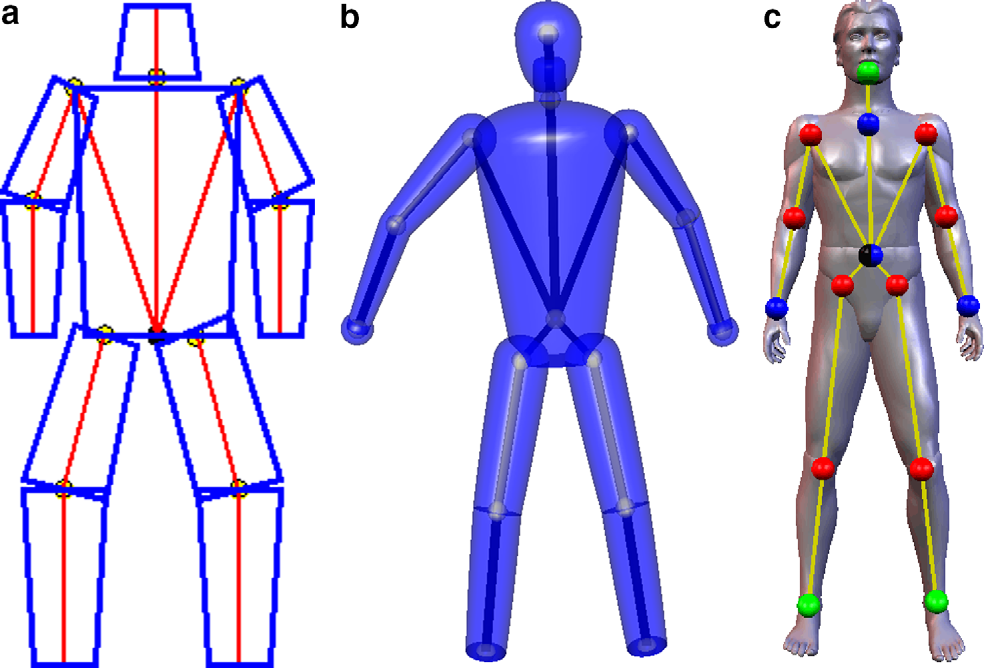
\includegraphics[width=0.5\textwidth]{assets/human_kinmodel.png}
%%\caption{Human shape models with kinematic model. (a) 2D model (Huang et al,IEEE 2002); (b) 3D volumetric model consisting of superquadrics (Kehl et al,Elsevier, 2006); (c) 3D surface model (Carranza et al, ACM, Inc., 2003).}
%\caption{Human shape models with kinematic model. (a) 2D model (b) 3D volumetric model (c) 3D surface model}
%\label{fig:humkinmodel}
%\end{figure}
\section{Human Pose Estimation}
\label{sec:humanpose}
  The surveys\cite{Moeslund2001231}\cite{Moeslund200690}\cite{Poppe20074} cited previously have investigated vision based human motion capture and analysis in general, however our particular focus is to use RGB-D sensors (presented in Section~\ref{ssec:rgbd_sensors}) to this purpose. Human pose estimation has traditionally suffered from two main problems
\begin{itemize}
\item Necessary to adopt an initialization pose.
\item Losing track after a few frames.
\end{itemize}
So alternative techniques which do not require to adopt an initialization pose and estimate pose from single depth images first appeared in the works of Shotton et al.,\cite{Shotton2011}.
\subsection{Estimation from Single Depth Images}
 The initial publication by the Xbox\cite{Kinect2014} team appeared in \cite{Shotton2011} where real time human pose estimation in parts using single depth images has been proposed. An extension of this work has been published recently by the Microsoft Computer vision research group\cite{Shotton2013}. This study proposes two approaches for human pose estimation which are capable of accurately predicting the 3D positions of body joints using single depth images without using any temporal information. The two methods also share their use of a very large, realistic, synthetic training corpus, generated by rendering depth images of humans. Each render is assigned randomly sampled parameters including body shape, size, pose, scene position, etc., thus generating quickly and cheaply hundreds of thousands of varied images with associated ground-truth (the body part label images and the set of 3D body joint positions). This enables to train deep forests, without the risk of overfitting, that can naturally handle a full range of human body shapes undergoing general body motions, self-occlusions, and poses cropped by the image frame. By using simple depth pixel comparison features, and parallelizable decision forests, both approaches could run in realtime on consumer hardware. The per-frame, per-joint proposals decribed in this study have been demonstrated to be usable even without tracking a full body model. This is crucial in HRI because there are scenarios in which the human might be sitting and there will be lot of occlusions. The key point in these algorithms is that they do background subtraction before the actual processing 
\begin{figure}[H]
\centering
\begin{subfigure}[b]{0.35\textwidth}
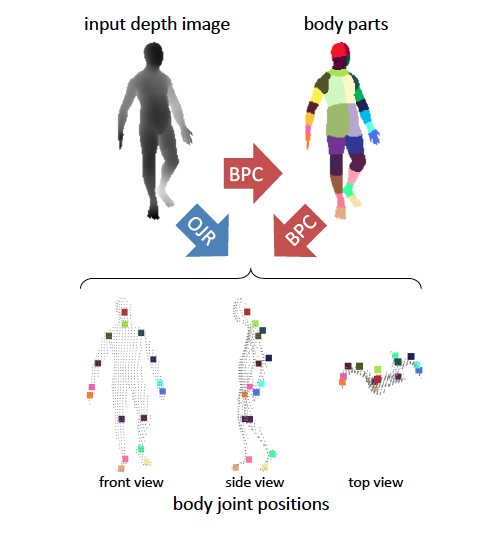
\includegraphics[width=\textwidth]{assets/kinect_approaches.png}
\caption{Human Pose estimation}
\label{fig:kinect_pose}
\end{subfigure}
\begin{subfigure}[b]{0.35\textwidth}
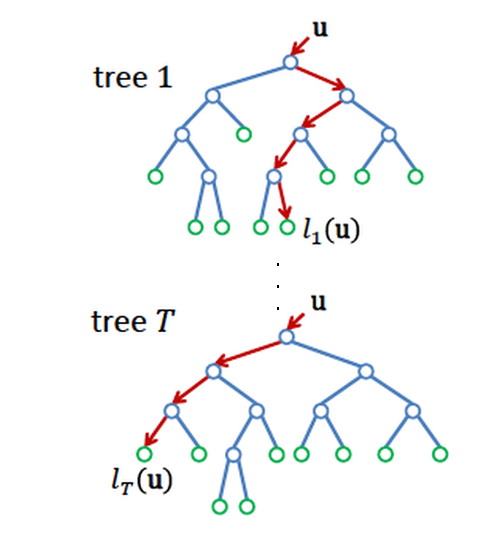
\includegraphics[width=\textwidth]{assets/forest.png}
\caption{Randomized Decision Forests}
\label{fig:decision_forests}
\end{subfigure}
\caption[Human pose estimation using single depth images]{Pose estimation using single depth images. {Adopted from \cite{Shotton2013}}}
\end{figure}
\subsubsection{Randomized Forests} A randomized forest\cite{Breiman01randomforests} is an ensemble of T decision trees as shown in Figure~\ref{fig:decision_forests}. Each tree consists of split nodes shown in blue and leaf nodes shown in green. The red arrows indicate the different paths that might be taken by different trees for a particular input $u$. Each split node contains a "weak learner" represented by its parameters $\theta = (\phi,\tau)$: the 2D offsets $\phi=\lbrace{ \delta_1,\delta_2 \rbrace}$ used for feature evaluation and a scalar threshold $\tau$. To make a prediction for pixel $u$ in a particular image starting at the root, traverse to a leaf by repeated evaluation of the weak learner function $h(u,\theta)$ given by
\begin{equation}
\label{eqn:weak_learner}
h(u,\theta) = [ f(u;\phi_n) \geq \tau_n ]
\end{equation} 
 
\subsubsection{Body Part Classification} The first approach employs an intermediate body parts representation, designed so that an accurate per-pixel classification of the parts will localize the joints of the body. It transforms the pose estimation problem into one that can be readily solved by classification algorithms. For the classification, \emph{31} body parts are defined: LU/RU/LW/RW head, neck, L/R shoulder, LU/RU/LW/RW arm, L/R elbow, L/R wrist, L/R hand, LU/RU/LW/RW torso, LU/RU/LW/RW leg, L/R knee, L/R ankle, and L/R foot (Left, Right, Upper, Lower). The classification forest used for Body Part Classification(BPC) uses a probability mass function(PMF) - $p_l(c)$ over body parts $c$ as the prediction model. The classification forest helps achieve the per-pixel classification by storing a distribution $p_l(c)$ over the discrete body parts $c$ at each leaf $l$. For a given input pixel $u$, the tree is descended to reach leaf $l = l(u)$ and the distribution $p_l(c)$ is retrieved. The distributions are averaged together for all trees in the forest to give the final classification as
\begin{equation}
p(c\vert \textbf{u}) = \frac{1}{T}\sum_{l\in L(\textbf{u})} p_l(c)
\label{eqn:bpc_dist}
\end{equation}
Where $p_l(c)$ is PMF at the leaf node corresponding to body part $c$, $u$ is input pixel and $T$ is number of decision trees. The image space predictions are next re-projected into world space. The re-projection function is denoted as $x(u) = (x(u); y(u); z(u))^\text{T}$. Conveniently, the known $z(u)$ from the calibrated depth camera allows to compute $x(u)$ and $y(u)$ trivially. The body parts inherently lie on the surface of the body, thus a learned per-joint vector ${\zeta_j} = (0,0,\zeta_j)^\text{T}$ is used to push back the re-projected pixel surface positions into the world to better align with the interior joint position: $x_j(u) = x(u) + {\zeta_j}$. The algorithm for BPC is described in Algorithm~\ref{alg:bpc} \\

\begin{algorithm}
 initialize ${X_j}^{BPC}$ = $\emptyset$; for all joints $j$ \;
 \ForAll{foreground pixels $u$ in the test image} { 
   evaluate forest to reach leaf nodes $L(u)$ \;
   evaluate distribution $p(c\vert u)$ using Eqn~\ref{eqn:bpc_dist} \;
   compute 3D pixel position $x(u) = (x(u); y(u); z(u))^\text{T}$ \;
   \ForAll{joints $j$}{
    compute pushed-back position $x_j(u)$ \;
    lookup relevant body part $c(j)$\;
    compute weight $w$ as $p(c = c(j)\vert u)$.$z^2(u)$\;
    add vote $(x_j(u);w)$ to set ${X_j}^{BPC}$ \;
    }
  }
 \Return set of votes ${X_j}^{BPC}$ for each joint $j$ \;
 \caption{Body part classification voting}
 \label{alg:bpc}
\end{algorithm}

\subsubsection{Offset Joint Regression} The second approach presented in \cite{Shotton2013} directly regresses the positions of body joints. The ground truth labels required for this approach are simply the ground truth 3D joint positions which are recorded during the mesh skinning process. In this approach \emph{16} body joints are defined: head, neck, L/R shoulder, L/R elbow, L/R wrist, L/R hand, L/R knee, L/R ankle, and L/R foot. The regression forest used for Offset Joint Regression (OJR) uses a set of weighted relative votes $V_{lj}$ for each joint $j$. At each leaf node $l$ a distribution over the relative 3D offset from the re-projected pixel coordinate $x(u)$ to each body joint $j$ of interest is stored. Each pixel can thus potentially cast votes to all joints in the body, and unlike BPC, these votes may differ in all world space coordinates and thus directly predict interior rather than surface positions. The distribution at the leaf node is represented using a \emph{small} set of 3D \emph{relative vote} vectors $\Delta_{ljk} \in \Re^3$. The subscript $l$ denotes the leaf node, $j$ denotes a body joint and $k \in \lbrace 1,...,K \rbrace$ denotes the maximum number of relative votes allowed. A confidence weight $w_{ljk}$ is associated with each vote and it is critical for the accuracy. The set of relative votes for joint $j$ at the node $l$ is denoted as $V_{lj}={{\lbrace (\Delta_{ljk},w_{ljk}) \rbrace}^K}_{k=1}$. In order to improve the speed, $N_{sub}$ samples could be obtained from ${X_j}^{OJR}$ by either random sampling or picking top $N_{sub}$ samples from it. The OJR algorithm is shown in Algorithm~\ref{alg:ojr}

\begin{algorithm}
 initialize ${X_j}^{OJR}$ = $\emptyset$; for all joints $j$ \;
 \ForAll{foreground pixels $u$ in the test image} { 
   evaluate forest to reach leaf nodes $L(u)$ \;
   compute 3D pixel position $x(u) = (x(u); y(u); z(u))^\text{T}$ \;
   \ForAll{leaves $l \in L(u)$}{
     \ForAll{joints $j$}{
       lookup weighted \emph{relative} vote set $V_{lj}$ \;
         \ForAll {$(\Delta_{ljk},w_{ljk})\in V_{lj}$}{
           compute \emph{absolute} position $x=x(u)+\Delta_{ljk}$ \;
           compute weight $w$ as $w_{ljk}.z^2(u)$ \;
           add vote $(x,w)$ to set ${X_j}^{OJR}$ \;
         }
     }
   }
  }
  sub-sample ${X_j}^{OJR}$ to contain at-most $N_{sub}$ votes \;
  \Return sub-sampled set of votes ${X_j}^{OJR}$ for each joint $j$ \;
 \caption{Offset joint regression voting}
 \label{alg:ojr}
\end{algorithm}

\subsubsection{One-Shot Model Fitting: The Vitruvian Manifold}
	Both \emph{BPC} and \emph{OJR} used one, or more hypotheses for the positions of each body joint. However, these work did not enforce kinematic constraints such as limb lengths, and are not able to disambiguate which hypotheses to stitch together into a coherent skeleton. In the work on Vitruvian Manifold \cite{Sharp2012} these concerns are addressed by fitting an articulated skeleton model to the observed data. A standard way to represent such an articulated skeleton is a global transformation (rotation, translation, scale) and then a hierarchical kinematic tree of relative transformations. In these transformations, the translation relative to the parent might be fixed (representing fixed limb lengths) but the rotation is parameterized(representing hinge joints). Given the kinematic hierarchy of transformations, linear blend skinning is used to generate a surface mesh of the body. It is standard to use Iterated Closest Point(ICP) algorithm to fit the parameters. Unfortunately, ICP requires a good initialization, and can take many iterations to converge. In the Vitruvian Manifold paper\cite{Sharp2012}, ‘One-Shot’ pose estimation is proposed whereby a good model fit is achieved by inferring these correspondences directly from the test image, and then performing only a single optimization of the model parameters. The BPC classification forest is extended for this purpose to predict at each pixel the corresponding vertex on the surface of the mesh model in a canonical pose (the so-called Vitruvian Manifold). The forests effectively become regression forests over this manifold, and allow a dense estimate of correspondence across the test image, without any initialization. Taking these correspondences and optimizing the model parameters resulted in most cases in a very accurate fit of the articulated skeleton to the observed data at low computational cost. An illustration of this approach is shown in Figure~\ref{fig:vitruvian}

\begin{figure}[H]
\centering
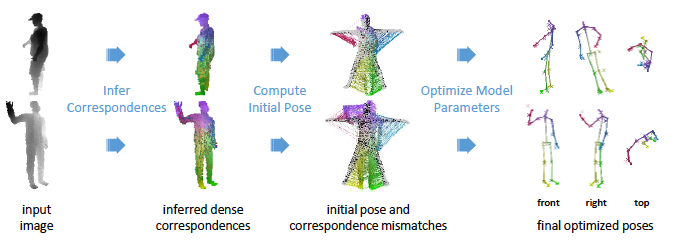
\includegraphics[width=\textwidth]{assets/vitruvian_manifold.png}
\caption[Pose Estimation pipeline in the vitruvian manifold algorithm]{Pose Estimation pipeline in the vitruvian manifold algorithm.{Adopted from \cite{Sharp2012}}}
\label{fig:vitruvian}
\end{figure}

\subsection{Estimation using both Depth and RGB image}
Unlike the approaches used in the Kinect SDK, the approach presented in \cite{Buys201439} uses both the depth and color(RGB-D) data for human body detection and pose estimation using a customizable human kinematic model. Other merits include the requirement of less training data and open source nature of this approach. 
\begin{figure}[H]
\centering
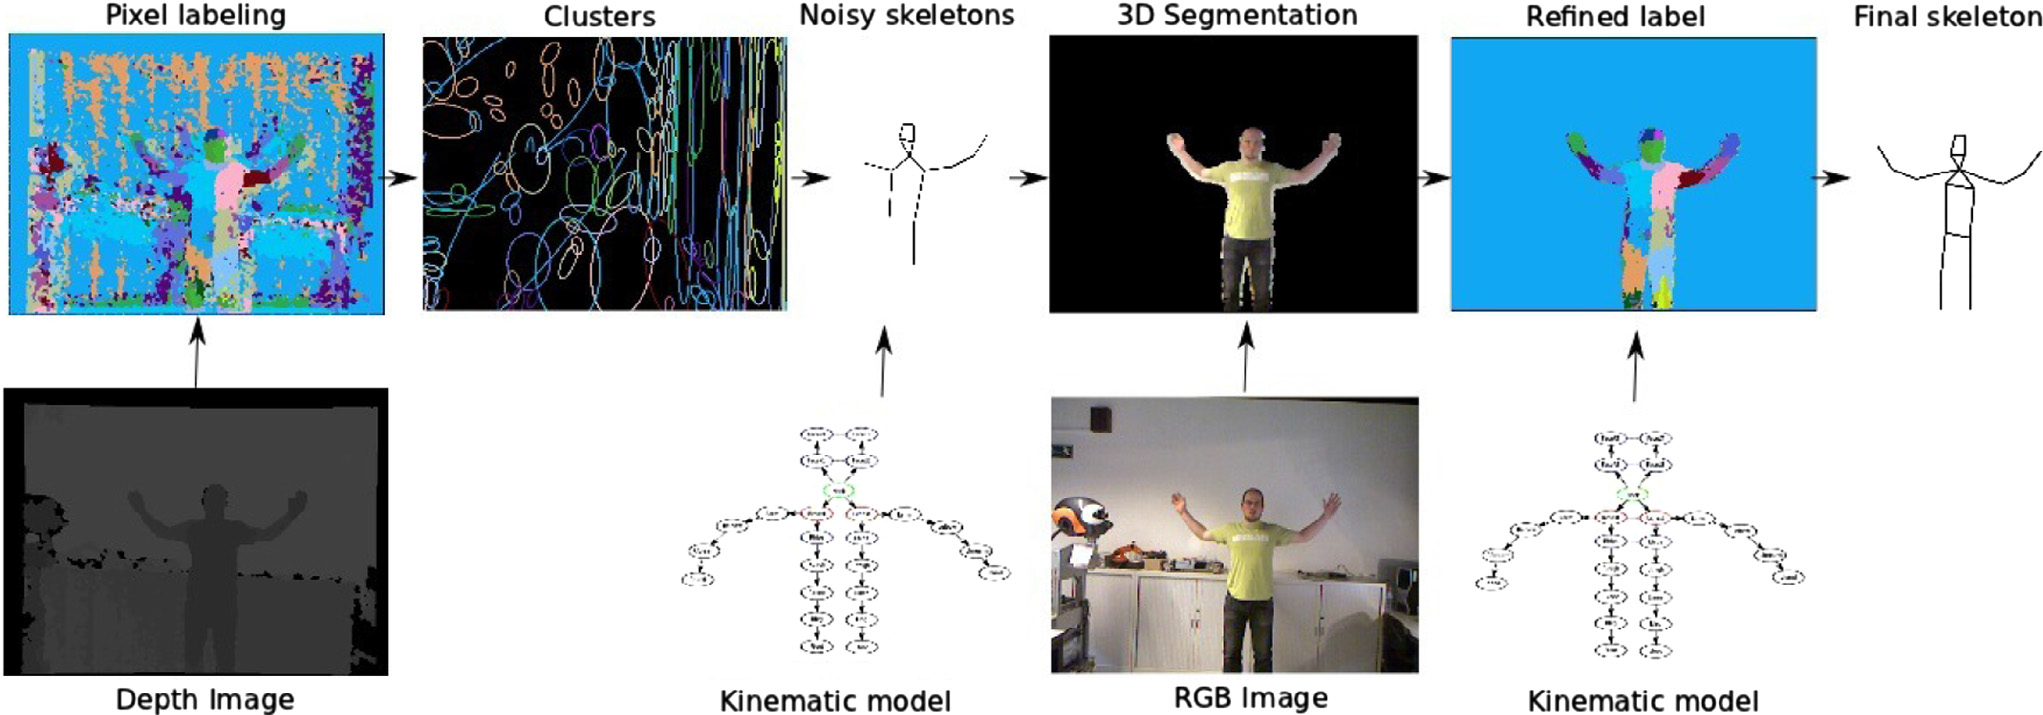
\includegraphics[width=\textwidth]{assets/adaptable_system_rgbd.png}
\caption[Adaptable system for human body detection and pose estimation]{Adaptable system for human body detection and pose estimation. {Adapted from \cite{Buys201439}}}
\label{fig:adaptable_rgbd}
\end{figure}

The goal of this approach is to output the 3D locations of the human body parts that are predefined in a kinematic model using the data received from an RGB-D sensor. The higher level process flow diagram of the system is shown in Figure~\ref{fig:adaptable_rgbd}. To start with, for a single depth map frame, per-pixel labeling is done as if each pixel is belonging to a single body part using the similar approach described in\cite{Shotton2011}. However the principal difference is that no \emph{background subtraction} or fixed-pose initialization step before pixel labeling. The initial result of pixel labels are very noisy. Hence a body part proposal step is followed which smooths the labels and clusters a more robot part estimates. Using the statistical inference of the part estimates, a search for feasible kinematic trees is conducted during the kinematic tree search step. This result in the person detections and noisy skeletonization. However there would be missing body parts and poor localization. In order to improve the obtained estimate, a second iteration of per-pixel body part labeling, body part proposal and kinematic tree search is performed based on the new estimate of the pixels actually belonging to the person being detected. An appearance model is estimated online for segmentation refinement step. This is done in order to obtain a new estimate of which pixel actually belong to the person being detected. The noisy initial estimate obtained during the first iteration is used as a seed for color and depth-based segmentation that retrieves missing body parts and better localizes existing parts. This process can be used for multiple people among clutter and occlusion. By running a second iteration a more robust and accurate human body pose estimate is obtained. This algorithm has been implemented as part of the PCL\cite{RusuPCL11} library under the name \emph{People's library}.

\section{Gesture Recognition}
	Understanding of human motion is not complete if the gesture of the human could not be understood. The next step after the human pose is tracked is to recognise the gesture. Hidden Markov models (HMM) which had been widely used for speech recognition\cite{Rabiner1990} also inspired to be used for the gesture recognition applications. The HMM model is generated for each motion primitives and Viterbi algorithm is used to find the optimum sequence of the states given a set of observations. During the recognition step a likelihood function is used on the segmented motion pattern against each HMM and the motion primitive corresponding to HMM with large likelihood is selected as shown in Figure~\ref{fig:hmm}. Auto segmentation of arm motion and recognition of motion patterns using angular velocity data obtained by IMU sensors and the Wii remote using HMM has been demostrated in \cite{Aoki2013}. 
\begin{figure}[H]
\centering
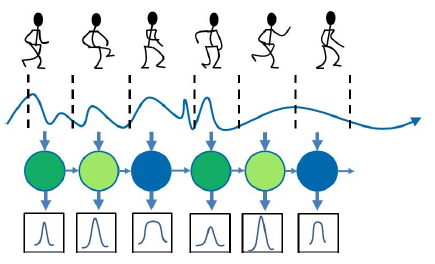
\includegraphics[width=0.3\textwidth]{assets/HMM.png}
\caption[HMM motion modeling]{HMM motion modeling. {Adapted from \cite{Aoki2013}}}
\label{fig:hmm}
\end{figure}
	In the publication by Microsoft research\cite{KinectCV2013}, a background study on various algortihms used for human activity analysis is presented. Recently\cite{KinectSDK2014} data-driven machine learning approaches like neural networks, Support vector machines, clustering, decision trees and bayesian networks are being exploited to this purpose. In \cite{KinectSDK2014}, an Adaptive Boosting algorithm\cite{Freund1997119} which is one of the top 10 data mining algorithms, is used to efficiently detect the gestures. The system involves a training phase in which the desired gestures are captured and tagged. These tagged gestures will be used by a gesture detector trainer which will generate a set of training examples $S=\lbrace \lbrace x_n,y_n \rbrace,\ n=1,\cdots,N \vert x_n\in X,y_n\in Y, X=\text{skeleton},Y=\lbrace -1,+1 \rbrace\rbrace$, associated data and set of weak classifiers $h_t$ and it learns the confidence $\alpha_t$ for $h_t$. The training results are stored in files and will be used by the gesture detector to perform per-frame classification of the data using $(h_t,\alpha_t)$. This approach has been proved to be robust with accuracy as high as 94.9\%. The general algorithm of Adaboost is shown in Algorithm~\ref{alg:adaboost}. \\
\begin{algorithm}[H]
 \label{alg:adaboost}
\KwData{$N$ labeled training samples: $S$}
For{$t$=$1,2,\cdots T$}{
	Weak learner $L$ selects weak classifier $h_t$ from pool\;
	Calculate confidence $\alpha_t$ for $h_t$\;
	Emphasize training examples that do not agree with $h_t$\;
}
\Return Strong classifier $H$ such that $H(x)=sign(\sum_{t=1}^{T}\alpha_t\cdot h_t(x))$
 \caption{Adaptive Boosting algorithm}
\end{algorithm}